\section{So sánh và đánh giá tổng thể các mô hình}\label{sec:compare}

\subsection{Bảng so sánh hiệu năng}\label{sec:final_test}
Cả bốn mô hình được so sánh ở cấu hình cuối cùng: 19 đặc trưng gốc, class weight, siêu tham số đã tuning và ngưỡng tối ưu F1 chọn trên xác suất out-of-fold. Tập test (1.409 khách hàng, 374 rời bỏ) chỉ được dùng một lần ở bước này.

\begin{table}[H]
\centering
\small
\begin{adjustbox}{max width=\textwidth}
\begin{tabular}{|l|c|c|c|c|c|c|c|c|}
\hline
\textbf{Mô hình} & \textbf{Ngưỡng} & \textbf{Accuracy} & \textbf{Precision} & \textbf{Recall} & \textbf{F1} & \textbf{ROC-AUC} & \textbf{PR-AUC} & \textbf{TP / FN / FP} \\
\hline
\textbf{XGBoost} & 0,57 & 0,771 & 0,550 & \textbf{0,749} & \textbf{0,634} & \textbf{0,846} & \textbf{0,662} & 280 / 94 / 229 \\
\hline
Decision Tree & 0,60 & 0,775 & 0,559 & 0,719 & 0,629 & 0,835 & 0,624 & 269 / 105 / 212 \\
\hline
Random Forest & 0,60 & \textbf{0,778} & \textbf{0,566} & 0,695 & 0,624 & 0,843 & 0,651 & 260 / 114 / 199 \\
\hline
Logistic Regression & 0,60 & 0,762 & 0,539 & 0,706 & 0,611 & 0,842 & 0,633 & 264 / 110 / 226 \\
\hline
\end{tabular}
\end{adjustbox}
\caption{So sánh hiệu năng các mô hình trên tập test (Precision, Recall, F1 tính cho lớp rời bỏ)}
\label{tab:final_test}
\end{table}

\begin{figure}[H]
\centering
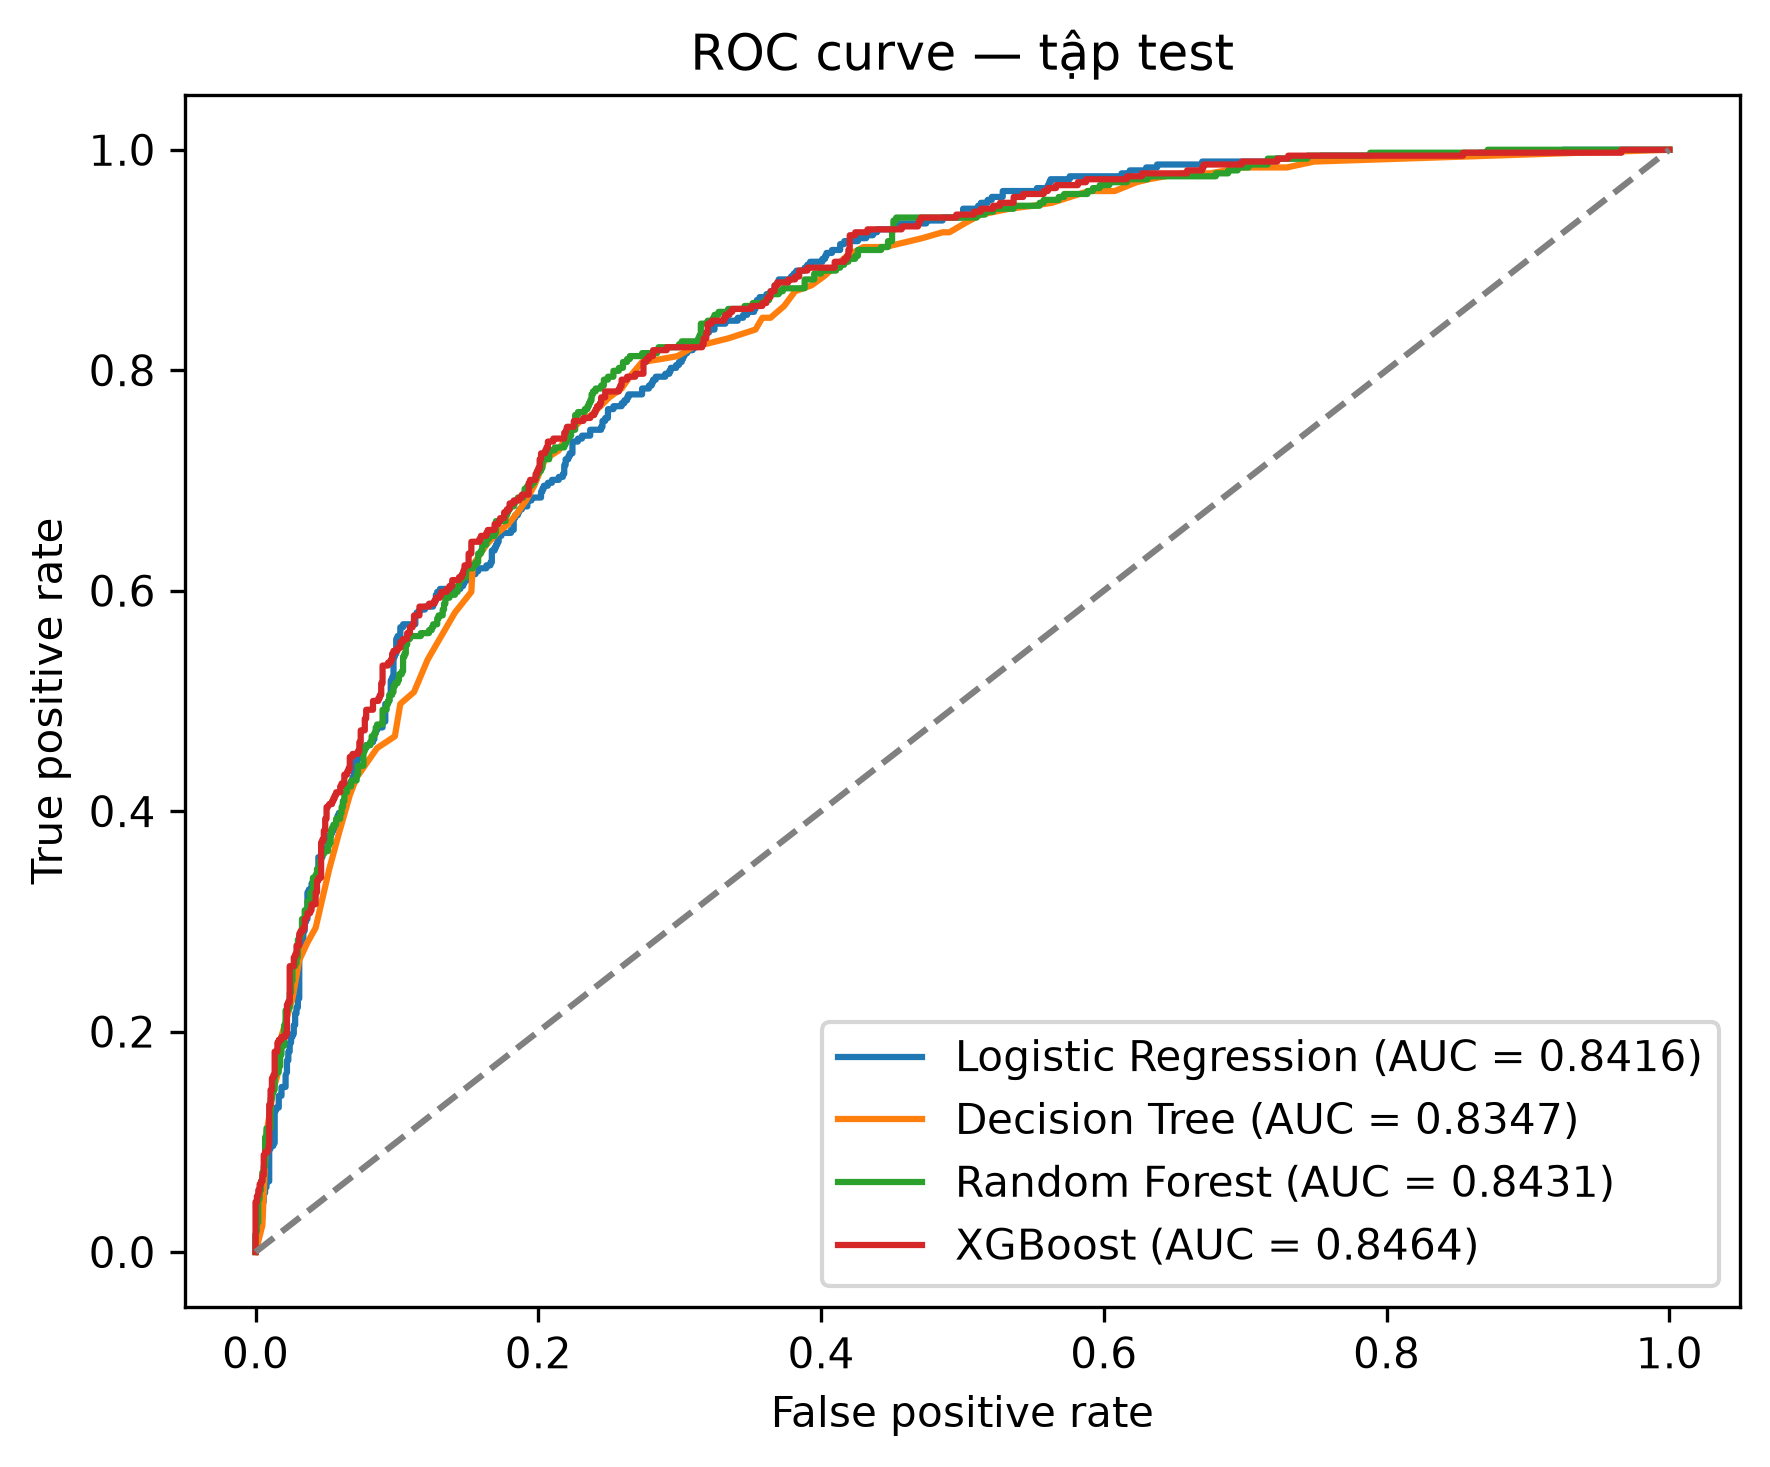
\includegraphics[width=0.49\textwidth]{img/final_roc.png}
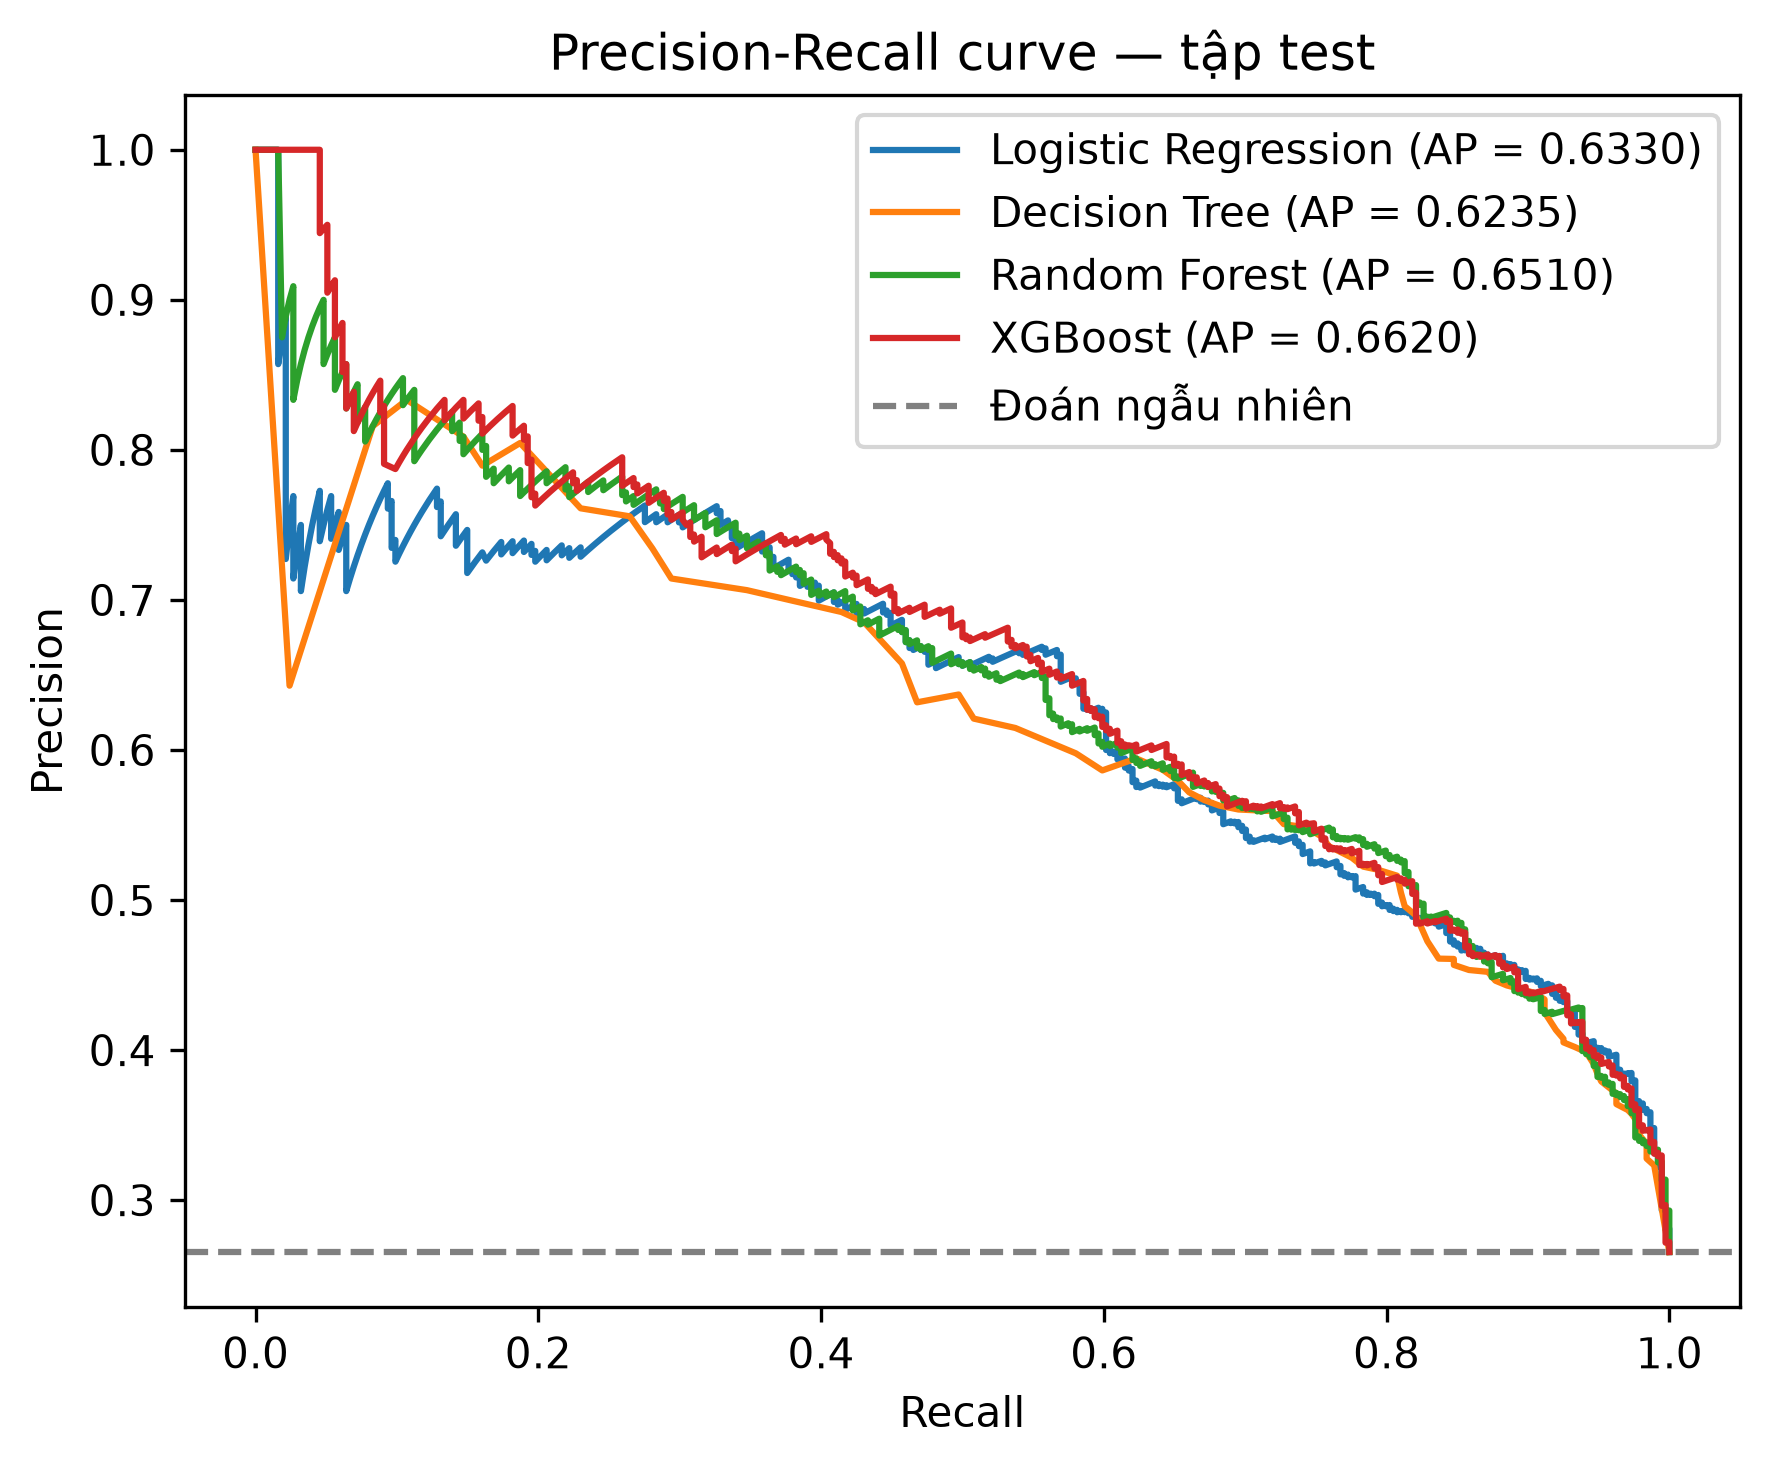
\includegraphics[width=0.49\textwidth]{img/final_pr.png}
\caption{Đường ROC (trái) và Precision--Recall (phải) của bốn mô hình trên tập test}
\end{figure}

\subsection{Phân tích so sánh}

\paragraph{Hiệu năng tổng thể}
\textbf{XGBoost} đạt kết quả tốt nhất ở F1 (0,634), Recall (0,749), ROC-AUC (0,846) và PR-AUC (0,662), khớp với lựa chọn dựa trên cross-validation trước khi xem tập test. Tuy nhiên khoảng cách giữa bốn mô hình rất nhỏ: F1 nằm trong khoảng 0,611--0,634 và ROC-AUC trong khoảng 0,835--0,846. Với 374 khách hàng rời bỏ trong tập test, chênh lệch F1 cỡ 0,02 có thể chỉ là nhiễu.

\paragraph{Đánh đổi Precision -- Recall}
Mỗi mô hình có điểm mạnh khác nhau ở lớp rời bỏ:
\begin{itemize}
    \item \textbf{XGBoost} có Recall cao nhất (0,749), bỏ sót ít khách hàng rời bỏ nhất (94).
    \item \textbf{Random Forest} có Precision (0,566) và Accuracy (0,778) cao nhất, ít cảnh báo nhầm nhất (199): phù hợp khi nguồn lực chăm sóc khách hàng hạn chế.
    \item \textbf{Decision Tree} cân bằng giữa hai mô hình trên với F1 0,629, nhưng khả năng xếp hạng (ROC-AUC, PR-AUC) thấp nhất.
    \item \textbf{Logistic Regression} có F1 thấp nhất (0,611) nhưng ROC-AUC (0,842) gần ngang các mô hình ensemble.
\end{itemize}

\paragraph{Độ tin cậy của ước lượng}
Kết quả test khớp với cross-validation (xem các Mục~\ref{sec:lr}--\ref{sec:xgb}): ROC-AUC sai khác không quá 0,005, PR-AUC giảm 0,007--0,027. Mức giảm nhỏ này phản ánh việc siêu tham số và ngưỡng được chọn trên cùng các fold dùng để chấm điểm; với XGBoost chỉ là 0,009 PR-AUC. Ngưỡng tối ưu F1 trên tập train không phải lúc nào cũng tốt hơn 0,5 trên tập test: F1 tăng với XGBoost (0,627 lên 0,634) và Decision Tree, nhưng giảm với Random Forest (0,639 xuống 0,624) và Logistic Regression -- đường F1 khá phẳng quanh ngưỡng tối ưu (Mục~\ref{sec:exp5}).

\paragraph{Tác động của từng kỹ thuật}
\begin{figure}[H]
\centering
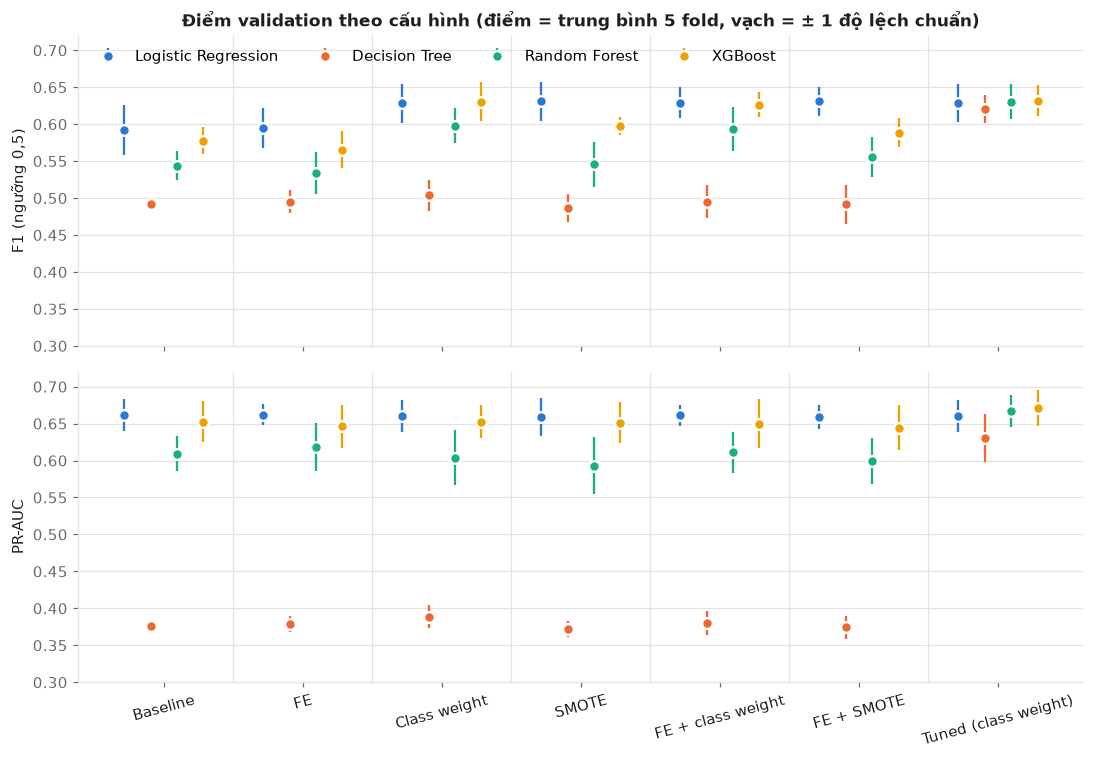
\includegraphics[width=0.85\textwidth]{img/nb_cv_overview.png}
\caption{F1 (ngưỡng 0,5) và PR-AUC validation của mọi cấu hình (chấm: trung bình 5 fold; vạch: $\pm$ 1 độ lệch chuẩn)}
\label{fig:cv_overview}
\end{figure}

\begin{table}[H]
\centering
\small
\begin{adjustbox}{max width=\textwidth}
\begin{tabular}{|l|c|p{9cm}|}
\hline
\textbf{Kỹ thuật} & \textbf{Tác động} & \textbf{Ghi chú} \\
\hline
Class weight & \textbf{Lớn} & F1 +0,036 đến +0,054 với LR, RF, XGBoost (5/5 fold); Recall tăng 0,16--0,26; đổi lại Precision giảm. \\
\hline
SMOTE & Trung bình & Tương đương class weight với LR; yếu hơn với mô hình cây. \\
\hline
Tuning & \textbf{Lớn với mô hình cây} & Decision Tree: F1 +0,12, PR-AUC +0,24; Random Forest: F1 +0,03, PR-AUC +0,06; không đổi với LR. \\
\hline
Feature Engineering & Không đáng kể & Mọi chênh lệch trong khoảng $\pm 0{,}012$, nhỏ hơn độ dao động giữa các fold. \\
\hline
Chọn ngưỡng & Nhỏ với F1 & +0,008 F1 trên CV, trên test lúc tăng lúc giảm; chủ yếu dùng để điều chỉnh cân bằng Precision--Recall. \\
\hline
\end{tabular}
\end{adjustbox}
\caption{Tác động của từng kỹ thuật (chi tiết ở Mục~\ref{sec:method})}
\label{tab:summary_effects}
\end{table}

Hai kỹ thuật mang lại cải thiện chính là \textbf{class weight} (giải quyết Recall thấp) và \textbf{tuning} (giải quyết overfitting của mô hình cây). Sau khi áp dụng cả hai, bốn mô hình đạt hiệu năng rất sát nhau (Hình~\ref{fig:cv_overview}, cột cuối), cho thấy giới hạn hiện tại nằm ở thông tin có trong dữ liệu hơn là ở lựa chọn thuật toán.

\paragraph{Tính diễn giải}
Các cách giải thích của bốn mô hình thống nhất về các yếu tố quan trọng nhất, đồng thời khớp với EDA (Mục~\ref{sec:eda}):
\begin{itemize}
    \item \textbf{\texttt{Contract}} và \textbf{\texttt{tenure}} đứng đầu ở mọi mô hình: hợp đồng theo tháng và khách hàng mới có nguy cơ rời bỏ cao nhất (Decision Tree dùng \texttt{Contract} ở nút gốc; Logistic Regression: mỗi độ lệch chuẩn \texttt{tenure} làm odds rời bỏ giảm còn 0,32 lần).
    \item \textbf{\texttt{InternetService}} (Fiber optic), các dịch vụ hỗ trợ (\texttt{TechSupport}, \texttt{OnlineSecurity}) và \textbf{\texttt{PaymentMethod}} (Electronic check) xếp tiếp theo.
    \item Các đặc trưng nhân khẩu học (giới tính, có vợ/chồng, người phụ thuộc) gần như không đóng góp.
\end{itemize}
Decision Tree có ưu thế về tính diễn giải (đọc trực tiếp các luật, Hình~\ref{fig:dt_structure}); Logistic Regression diễn giải được qua hệ số nhưng bị ảnh hưởng bởi đa cộng tuyến; Random Forest và XGBoost cần các công cụ như permutation importance.

\subsection{Kết luận}

\begin{table}[H]
\centering
\small
\begin{adjustbox}{max width=\textwidth}
\begin{tabular}{|l|c|c|c|c|}
\hline
\textbf{Tiêu chí} & \textbf{Logistic Regression} & \textbf{Decision Tree} & \textbf{Random Forest} & \textbf{XGBoost} \\
\hline
F1 lớp rời bỏ (test) & Thấp nhất & Cao & Trung bình & \textbf{Cao nhất} \\
\hline
Recall lớp rời bỏ & Trung bình & Cao & Thấp nhất & \textbf{Cao nhất} \\
\hline
Precision lớp rời bỏ & Thấp nhất & Cao & \textbf{Cao nhất} & Trung bình \\
\hline
Khả năng xếp hạng (ROC/PR-AUC) & Trung bình & Thấp nhất & Cao & \textbf{Cao nhất} \\
\hline
Hiệu năng khi chưa tuning & \textbf{Cao nhất} & Thấp nhất & Trung bình & Cao \\
\hline
Chống overfitting & \textbf{Tốt} & Cần tuning & Cần tuning & Tốt sau tuning \\
\hline
Tính diễn giải & Cao (hệ số) & \textbf{Cao nhất} (luật) & Thấp & Thấp \\
\hline
Chi phí tính toán & \textbf{Thấp} & \textbf{Thấp} & Cao & Trung bình \\
\hline
\end{tabular}
\end{adjustbox}
\caption{Đánh giá tổng hợp các mô hình theo từng tiêu chí}
\end{table}

\textbf{Mô hình cuối cùng} là \textbf{XGBoost đã tuning, class weight, ngưỡng 0,57}: F1 0,634, Recall 0,749, Precision 0,550, ROC-AUC 0,846, PR-AUC 0,662 trên tập test, phát hiện được 280/374 khách hàng rời bỏ so với khoảng một nửa ở cấu hình baseline. Không có mô hình nào vượt trội hoàn toàn: \textbf{Random Forest} phù hợp hơn khi cần ít cảnh báo nhầm; \textbf{Decision Tree} và \textbf{Logistic Regression} phù hợp khi cần giải thích rõ ràng cho bộ phận kinh doanh, với hiệu năng chỉ thấp hơn một chút.

\textbf{Bài học chính} từ các thực nghiệm:
\begin{enumerate}
    \item Với dữ liệu mất cân bằng, xử lý mất cân bằng (class weight) là bước mang lại cải thiện F1 lớn nhất và ổn định nhất.
    \item Mô hình cây cần kiểm soát độ phức tạp; tuning loại bỏ overfitting và giúp class weight phát huy tác dụng.
    \item Feature Engineering dựa trên các đặc trưng đã có không cải thiện hiệu năng, vì mô hình tự học được các ngưỡng và tương tác tương ứng.
    \item Chọn ngưỡng không giúp tăng F1 đáng kể nhưng là công cụ để điều chỉnh cân bằng Precision--Recall theo nhu cầu kinh doanh.
\end{enumerate}

\subsubsection{Ý nghĩa kinh doanh}
Các quan sát dưới đây là mối liên hệ thống kê, không phải quan hệ nhân quả:
\begin{itemize}
    \item Khách hàng hợp đồng theo tháng, mới sử dụng dịch vụ là nhóm rủi ro cao nhất; ưu đãi chuyển sang hợp đồng dài hạn có thể là đòn bẩy giữ chân.
    \item Khách hàng dùng Fiber optic nhưng không đăng ký TechSupport/OnlineSecurity có tỉ lệ rời bỏ cao; cần xem xét chất lượng dịch vụ và gói hỗ trợ đi kèm.
    \item Ngưỡng quyết định nên được chọn theo chi phí: ngưỡng tối ưu F1 (0,57) cân bằng Precision và Recall; nếu bỏ sót một khách hàng rời bỏ tốn kém hơn nhiều so với gửi nhầm một ưu đãi, ngưỡng F2 (0,37) phát hiện được 329/374 khách hàng rời bỏ với Precision 0,46.
\end{itemize}

\subsubsection{Hạn chế và hướng phát triển}
\begin{itemize}
    \item Bộ dữ liệu nhỏ (7.043 khách hàng) và là ảnh chụp tĩnh, không có thông tin hành vi theo thời gian.
    \item Siêu tham số và ngưỡng được chọn trên cùng các fold dùng để chấm điểm nên điểm cross-validation sau tuning hơi lạc quan; nested cross-validation sẽ cho ước lượng khách quan hơn.
    \item Chưa thực hiện so sánh các phương pháp Encoding/Scaling như kế hoạch ban đầu.
    \item Hướng phát triển: chọn ngưỡng theo hàm chi phí khi có số liệu kinh doanh, hiệu chỉnh xác suất, giải thích theo từng khách hàng bằng SHAP, thử LightGBM/CatBoost và triển khai mô hình dưới dạng API hoặc dashboard.
\end{itemize}
